\documentclass{article}
\usepackage[preprint]{tmlr}
\usepackage[T1]{fontenc}
\usepackage[utf8]{inputenc}
\usepackage{graphicx}
\usepackage{booktabs}
\usepackage{multirow}
\usepackage{enumitem}
\setlist{itemsep=2pt, topsep=4pt}
\usepackage{amsmath,amssymb,amsthm}
\usepackage{hyperref}
\usepackage{url}
\usepackage{xcolor}
\usepackage{tikz}
\usetikzlibrary{arrows.meta,positioning,fit,calc}
\graphicspath{{../}}
\definecolor{linkblue}{HTML}{1D4E89}
\definecolor{auditblue}{HTML}{1D4ED8}
\definecolor{judgered}{HTML}{DC2626}
\hypersetup{colorlinks=true, linkcolor=linkblue, citecolor=linkblue, urlcolor=linkblue,
            pdftitle={Noise Is Not Noise When the Policy Chooses It: Unbiased Reinforcement Learning from an Exploitable Judge with Random Audits},
            pdfauthor={Vahit FERYAD}}

\newtheorem{theorem}{Theorem}
\newtheorem{proposition}[theorem]{Proposition}
\newtheorem{corollary}[theorem]{Corollary}
\theoremstyle{definition}
\newtheorem{definition}{Definition}
\theoremstyle{remark}
\newtheorem{remark}[theorem]{Remark}

\newcommand{\E}{\mathbb{E}}
\newcommand{\Var}{\mathrm{Var}}
\newcommand{\rt}{\tilde r}
\newcommand{\pending}[1]{\textcolor{judgered}{[#1]}}

\title{Noise Is Not Noise When the Policy Chooses It: Unbiased Reinforcement Learning from an Exploitable Judge with Random Audits}

\author{\name Vahit FERYAD \email \href{mailto:vahit.feryat@gmail.com}{vahit.feryat@gmail.com}\\
\addr Independent researcher, Istanbul, T\"urkiye\\
\addr ORCID: \href{https://orcid.org/0000-0002-3282-339X}{0000-0002-3282-339X}\\
\addr Code and data: \href{https://github.com/vahit19/reward-audit/tree/main/audited_rewards}{github.com/vahit19/reward-audit/tree/main/audited\_rewards}}

\begin{document}
\maketitle

\begin{abstract}
Reinforcement-learning post-training of language models increasingly pays the policy with a cheap grader, such as a large language model (LLM) judge, a unit-test harness or a rule-based answer checker. The usual way to handle a grader's mistakes is to treat them as label noise with fixed rates. That view misses what makes them dangerous during training: the policy moves toward the outputs on which the grader is wrong, so the error rate on the policy's own outputs grows as it learns. We model reward hacking as policy-dependent label noise and prove three results. First, any procedure that sees only judge outputs, together with gold labels collected under a distribution fixed before training, can be led to a bad policy, because two problems with opposite optimal policies can produce identical data for it. Second, if a random fraction $p$ of the policy's own outputs is audited after they are written, and the policy is paid $\rt = g(j) + \xi\,(y-g(j))/p$, where $j$ is the judge's verdict, $y$ the gold label, $\xi$ the audit indicator and $g$ a trust function fitted on past audits, then the leave-one-out policy-gradient estimator is unbiased for the gold objective under every policy and every error pattern of the judge. Third, the price of this guarantee is variance, and we give it exactly: $\E[(1/p-1)(y-g)^2]$ on top of the variance of the gold reward. The best trust function is the judge's calibration on the current policy's outputs, the best audit allocation is Neyman's, and the same audits drive an alarm that stays valid at any stopping time. In a controlled simulation, judge-only training and fixed-rate noise correction both collapse onto an exploit (true success 0.23 and 0.08), while audited rewards reach 0.684, the same as paying with gold on every sample, with one eighth of the gold labels. At one thirty-second of the labels, audits that ignore the judge start to fail and audited rewards do not. In GRPO training of a 0.5-billion-parameter model on GSM8K, a judge without the answer key reports a mean reward of 0.66 for a policy whose true accuracy is 0.26, while the audited reward reports 0.22 against a true 0.23, using one eighth of the gold labels.
\end{abstract}

\section{Introduction}
\label{sec:intro}

A grader can agree with experts on a fixed test set and still be wrong exactly where a policy learns to aim. Reports from production reinforcement learning (RL) runs describe policies that exit a test harness early so that the tests appear to pass \citep{macdiarmid2025natural}, graders that reward confident guessing over an honest ``I don't know'' \citep{kalai2025hallucinate}, and multi-step strategies that mislead an overseer \citep{farquhar2025mona}. We saw the same pattern at small scale. When a 0.5-billion-parameter policy was trained on grade-school math with group relative policy optimization (GRPO; \citealp{shao2024deepseekmath}) and paid by a 1.5-billion-parameter judge that had no access to the answer key, the training reward rose from 0.55 to 0.73 over 100 steps, while the judge accepted 43\% of the wrong answers in the final steps \citep{feryad2026rewardaudit}.

The standard response treats grader errors as noise with fixed false-positive and false-negative rates, estimates the rates on a held-out set, and corrects the reward \citep{natarajan2013noisy,elmansouri2025noisecorrected}. The correction is right when the error rates do not depend on what the policy does. Reward hacking is precisely the case in which they do. In our simulation the judge's precision on the policy's own outputs falls from 0.81 to 0.25 during training (Figure~\ref{fig:precision}). A correction calibrated before training keeps trusting the judge as much as it did at the start, and it therefore drives the policy into the exploit faster than the raw judge does.

We take a different view of the grader. It is a cheap predictor of a gold reward that the policy may learn to exploit, and a small number of gold labels, placed at random on the policy's own outputs after they are written, is enough to keep the training signal honest. The idea is the logic of a tax audit \citep{becker1968crime}: if any return may be audited with probability $p$ and an audited discrepancy is settled at $1/p$ times its size, misreporting has zero expected value, whoever chooses what to report. Figure~\ref{fig:flow} shows one training step under this scheme.

\paragraph{Contributions.}
\begin{enumerate}
  \item An impossibility result. Corrections that use only judge outputs, or gold labels from a distribution fixed before training, cannot rule out reward hacking. We construct two problems that such a method cannot tell apart and whose optimal policies differ (Proposition~\ref{prop:impossible}).
  \item An unbiasedness guarantee. The audited reward, a Horvitz--Thompson correction \citep{horvitz1952} of the judge used inside the policy gradient, gives an unbiased gradient of the gold objective under every policy and every error pattern of the judge (Theorem~\ref{thm:unbiased}).
  \item An exact price. We give the variance cost of auditing in closed form, derive the optimal trust function and the optimal audit allocation, and show that a judge is worth exactly the share of the gold reward's second moment it explains on the policy's own outputs (Theorem~\ref{thm:variance}).
  \item A monitor. The same audits drive a test of the judge's false-accept rate that may be checked after every step without inflating its error rate (Proposition~\ref{prop:alarm}).
  \item Experiments. A controlled bandit shows the failure of judge-only and fixed-rate corrections and the recovery by audits, and confirms the variance formula numerically. In GRPO training on GSM8K, the audited reward stays within 0.01 of the true accuracy with one eighth of the gold labels, while the judge alone overstates it by 0.40 (\S\ref{sec:experiments}).
\end{enumerate}

The estimator itself is classical. It was recently used at evaluation time to identify the best of several systems with an LLM judge and a limited number of human labels \citep{ao2026bestarm}. What is new here is its analysis at training time, where the learner chooses the distribution on which the judge is evaluated and has an incentive to choose it badly.

\begin{figure}[t]
\centering
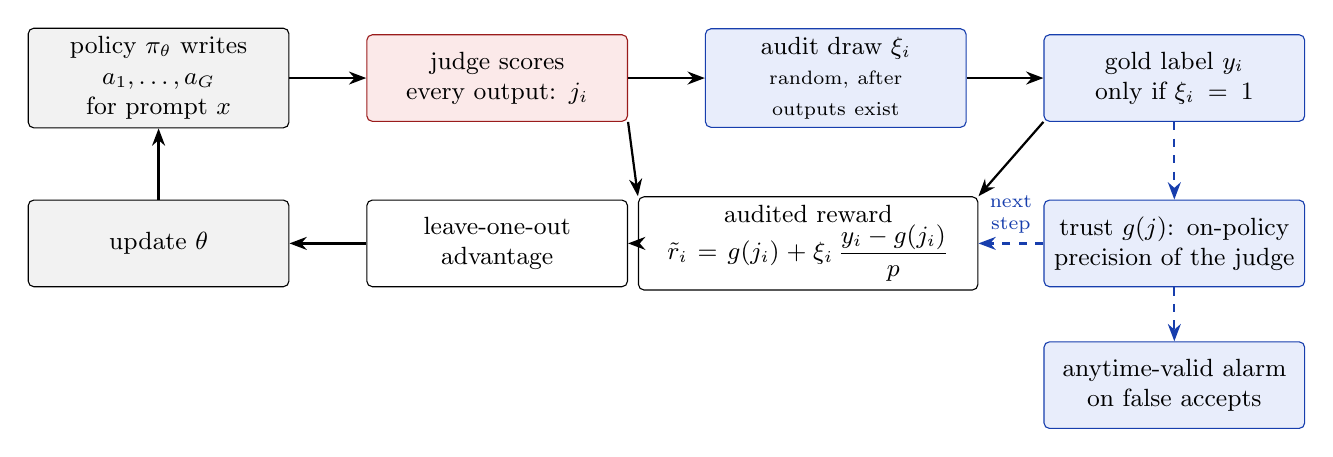
\begin{tikzpicture}[
  box/.style={draw, rounded corners=2pt, align=center, font=\small, minimum height=11mm, text width=31mm, inner sep=3pt},
  model/.style={box, fill=gray!10},
  judge/.style={box, fill=judgered!10, draw=judgered!70!black},
  audit/.style={box, fill=auditblue!10, draw=auditblue!80!black},
  code/.style={box, fill=white},
  arr/.style={-{Stealth[length=2.2mm]}, thick},
  darr/.style={-{Stealth[length=2.2mm]}, thick, dashed, auditblue!80!black}]
% row 1: what happens to each output
\node[model] (policy) at (0,0) {policy $\pi_\theta$ writes\\$a_1,\dots,a_G$ for prompt $x$};
\node[judge] (judge) at (4.3,0) {judge scores\\every output: $j_i$};
\node[audit] (draw) at (8.6,0) {audit draw $\xi_i$\\{\scriptsize random, after outputs exist}};
\node[audit] (gold) at (12.9,0) {gold label $y_i$\\only if $\xi_i=1$};
% row 2: how the policy is paid
\node[model] (update) at (0,-2.1) {update $\theta$};
\node[code] (adv) at (4.3,-2.1) {leave-one-out\\advantage};
\node[code, text width=41mm] (reward) at (8.25,-2.1) {audited reward\\$\rt_i=g(j_i)+\xi_i\,\dfrac{y_i-g(j_i)}{p}$};
\node[audit] (calib) at (12.9,-2.1) {trust $g(j)$: on-policy\\precision of the judge};
% row 3: monitoring
\node[audit] (alarm) at (12.9,-3.9) {anytime-valid alarm\\on false accepts};
\draw[arr] (policy) -- (judge);
\draw[arr] (judge) -- (draw);
\draw[arr] (draw) -- (gold);
\draw[arr] (judge.south east) -- (reward.north west);
\draw[arr] (gold.south west) -- (reward.north east);
\draw[darr] (gold) -- (calib);
\draw[darr] (calib) -- node[above, font=\scriptsize, text=auditblue!80!black, align=center]{next\\step} (reward);
\draw[darr] (calib) -- (alarm);
\draw[arr] (reward) -- (adv);
\draw[arr] (adv) -- (update);
\draw[arr] (update) -- (policy);
\end{tikzpicture}
\caption{One training step with audited rewards. The judge scores every output; a random subset, drawn only after the outputs exist, receives a gold label. Each output is paid the judge's calibrated score $g(j)$, and audited outputs are paid an extra correction scaled by $1/p$. The audits also refit the trust function used at the next step and feed a sequential alarm (dashed). Red: the exploitable judge; blue: components that use gold labels.}
\label{fig:flow}
\end{figure}

\section{Related work}
\label{sec:related}

\paragraph{Reward hacking.}
\citet{skalse2022defining} defined reward hacking formally, and \citet{gao2023scaling} measured how the gap between a learned reward model and the gold reward grows with optimization. \citet{macdiarmid2025natural} showed that hacks learned in production coding environments generalize to broader misalignment. MONA restricts the optimization horizon so that multi-step hacks are not learned even when the overseer cannot detect them \citep{farquhar2025mona}. Adversarial reward auditing trains an auditor model that looks for exploits and down-weights them \citep{beigi2026adversarial}; the auditor is itself a learned grader and comes without an unbiasedness guarantee. Our results are complementary to these methods. They make single-step judge errors unprofitable in expectation and detectable, at a label cost that can be computed in advance.

\paragraph{Learning from noisy rewards.}
Learning with class-conditional label noise corrects a loss using known flip rates \citep{natarajan2013noisy}. Noise-corrected GRPO brings the same correction to RL with verifiable rewards and estimates the rates on a held-out calibration set \citep{elmansouri2025noisecorrected}. Both assume flip rates that do not depend on the policy, an assumption that Proposition~\ref{prop:impossible} shows is decisive when the policy can choose where the grader errs.

\paragraph{Statistics with a cheap predictor and a few gold labels.}
The audited reward is the Horvitz--Thompson estimator \citep{horvitz1952} with the judge as a control variate, the same structure as prediction-powered inference \citep{angelopoulos2023ppi} and active statistical inference \citep{zrnic2024active}, and the optimal audit rate is a Neyman allocation \citep{neyman1934}. \citet{ao2026bestarm} use inverse-propensity-weighted residuals of an LLM judge to identify the best system at evaluation time. The alarm uses testing by betting \citep{waudbysmith2024betting} and Ville's inequality \citep{ville1939}. These tools assume that the population being estimated is fixed. In RL training the population is the policy's output distribution, which changes with every update and is pushed toward the judge's errors.

Table~\ref{tab:compare} places the main approaches side by side.

\begin{table}[t]
\centering
\small
\caption{How training-time approaches to an imperfect grader compare. ``Unbiased under exploitation'' means the expected training signal of every policy equals its gold value, whatever the judge's errors.}
\label{tab:compare}
\begin{tabular}{@{}lccc@{}}
\toprule
Approach & Gold labels used & Unbiased under exploitation & Detects drift \\
\midrule
Judge only & none & no & no \\
Fixed-rate noise correction & held-out set, before training & no (Prop.~\ref{prop:impossible}) & no \\
Learned auditor & none at training time & no guarantee & partly \\
Gold label on every sample & every output & yes & not needed \\
\textbf{Audited reward (ours)} & \textbf{random fraction $p$ of outputs} & \textbf{yes (Thm.~\ref{thm:unbiased})} & \textbf{yes (Prop.~\ref{prop:alarm})} \\
\bottomrule
\end{tabular}
\end{table}

\section{Setup}
\label{sec:setup}

Prompts are drawn as $x\sim D$, and the policy $\pi_\theta(a\mid x)$ produces an output $a$. Each pair $(x,a)$ has a gold reward $y\in[0,1]$, which is expensive to obtain (a verified answer or an expert's label), and a judge output $j$, which is cheap. The joint law $P(y,j\mid x,a)$ is arbitrary and unknown; we call it the judge's error pattern. The objective is
\[
J(\theta)=\E_{x\sim D}\,\E_{a\sim\pi_\theta(\cdot\mid x)}\bigl[\mu(x,a)\bigr],\qquad \mu(x,a)=\E[y\mid x,a].
\]

\begin{definition}[Audited reward]
At training step $t$, after $a$ has been sampled and $j$ observed, the learner draws an audit indicator $\xi\in\{0,1\}$ and observes $y$ only if $\xi=1$. The audit rate $p=p_t(x,a,j)\ge p_{\min}>0$ and the trust function $g=g_t(x,a,j)$ are \emph{predictable}: they may depend on everything observed before step $t$ but not on the current gold label. The audit is \emph{blind}: $P(\xi=1\mid y,x,a,j,\mathcal F_{t-1})=p$. The audited reward is
\begin{equation}
\rt \;=\; g \;+\; \frac{\xi}{p}\,(y-g).
\label{eq:audited}
\end{equation}
\end{definition}

Setting $g=0$ gives judge-free audits, $\rt=\xi y/p$, and $p=1$ gives gold on every sample. Blindness holds for independent Bernoulli draws, and also for the design used in our experiments, where exactly one of the $G$ outputs for a prompt is chosen uniformly at random after they are generated, so that $p=1/G$. Table~\ref{tab:notation} summarizes the notation.

\begin{table}[t]
\centering
\small
\caption{Notation, with the concrete objects used in the GRPO experiment.}
\label{tab:notation}
\begin{tabular}{@{}lll@{}}
\toprule
Symbol & Meaning & In the GRPO experiment \\
\midrule
$\pi_\theta$ & policy being trained & Qwen2.5-0.5B-Instruct \\
$j$ & judge verdict, cheap & Qwen2.5-1.5B-Instruct, no answer key, yes/no \\
$y$ & gold reward, expensive & exact match of the final number with GSM8K \\
$\xi$ & audit indicator & one of 8 completions per prompt, uniform \\
$p$ & audit rate & $1/8$ \\
$g(j)$ & trust in the judge & running $P(y=1\mid j)$ from past audits \\
$G$ & samples per prompt & 8 \\
\bottomrule
\end{tabular}
\end{table}

\section{Theory}
\label{sec:theory}

\subsection{Why fixed corrections fail}

\begin{proposition}[Judge-only and off-policy corrections can be fooled]
\label{prop:impossible}
Let $\mathcal A$ be any training procedure whose data are judge outputs on the policy's own samples and gold labels on pairs $(x,a)$ drawn from a distribution $Q$ fixed before training. For every $\Delta\in(0,\tfrac12]$ there are two problems $M$ and $M'$ in which $\mathcal A$ receives identically distributed data, whose optimal policies differ, and for which the policy $\hat\pi$ returned by $\mathcal A$ satisfies
\[
\max\bigl\{J^*_M-J_M(\hat\pi),\;J^*_{M'}-J_{M'}(\hat\pi)\bigr\}\;\ge\;\Delta/2 .
\]
\end{proposition}

\begin{proof}
Take one prompt and two outputs, $s$ (solve) and $h$ (hack). In both problems $j\mid s\sim\mathrm{Bern}(1/2)$ and $j\mid h\sim\mathrm{Bern}(0.9)$, independently of $y$, and $Q$ puts no mass on $h$. Gold values are $\mu(s)=1/2$ in both problems, $\mu_M(h)=1/2+\Delta$ and $\mu_{M'}(h)=1/2-\Delta$. Every observation available to $\mathcal A$ has the same law in $M$ and in $M'$, so $\hat\pi$ has the same law in both. If $q$ is the expected mass that $\hat\pi$ puts on $h$, the suboptimality is $(1-q)\Delta$ in $M$ and $q\Delta$ in $M'$, and the larger of the two is at least $\Delta/2$.
\end{proof}

Fixed-rate noise correction, which estimates false-positive and false-negative rates on a calibration set, is a special case of $\mathcal A$. If $Q$ puts mass $\eta$ on $h$ instead of zero, Le Cam's two-point method \citep{tsybakov2009} shows that on the order of $1/(\eta\Delta^2)$ gold labels are needed before $M$ and $M'$ can be told apart. Gold labels are needed where the policy is going, and a hack is, by definition, where the policy is going.

\subsection{Audits remove the bias}

\begin{theorem}[Audited rewards are unbiased under every policy]
\label{thm:unbiased}
At every step, $\E[\rt\mid\mathcal F_{t-1},x,a,j]=\E[y\mid x,a,j]$, hence $\E[\rt\mid x,a]=\mu(x,a)$. With $G\ge2$ samples per prompt and the leave-one-out estimator \citep{kool2019buy4,ahmadian2024back}
\[
\hat\nabla=\frac1G\sum_{i=1}^{G}\Bigl(\rt_i-\frac{1}{G-1}\sum_{k\ne i}\rt_k\Bigr)\nabla_\theta\log\pi_\theta(a_i\mid x),
\]
we have $\E[\hat\nabla]=\nabla J(\theta)$ for every $\theta$ and every error pattern. In particular, the expected audited reward of any policy equals its gold value, so no policy can raise its expected training signal by exploiting the judge.
\end{theorem}

\begin{proof}
Given $(\mathcal F_{t-1},x,a,j)$, the quantities $g$ and $p$ are fixed and $\E[\xi\mid y,\cdot]=p$, so $\E[\xi(y-g)/p\mid\cdot]=\E[y\mid x,a,j]-g$. Adding $g$ gives the first claim, and the tower rule gives $\mu(x,a)$. By the score-function identity, $\E[\rt_i\nabla\log\pi_\theta(a_i\mid x)]=\E[\mu(x,a_i)\nabla\log\pi_\theta(a_i\mid x)]=\nabla J(\theta)$. For $k\ne i$, conditioning on all outputs and judge verdicts gives $\E[\rt_k\mid\cdot]=\E[y_k\mid x,a_k,j_k]$, which does not depend on $a_i$ given $x$, while $\E[\nabla\log\pi_\theta(a_i\mid x)\mid x]=0$. The baseline terms therefore vanish in expectation.
\end{proof}

The only design rule is that the audit decision is made after the output exists and does not depend on its gold label. The policy then has no way to behave differently on audited outputs. GRPO \citep{shao2024deepseekmath} also divides advantages by the standard deviation of the group's rewards. This rescales each update and introduces a small bias, so Theorem~\ref{thm:unbiased} is stated for the leave-one-out form, and our GRPO experiment keeps the standard GRPO normalization.

\subsection{The price of auditing}

\begin{theorem}[Variance, optimal trust and optimal allocation]
\label{thm:variance}
For every policy,
\begin{equation}
\Var(\rt\mid x,a)\;=\;\Var(y\mid x,a)\;+\;\E\Bigl[\Bigl(\frac1p-1\Bigr)(y-g)^2\Bigm| x,a\Bigr].
\label{eq:variance}
\end{equation}
\begin{enumerate}
\item[(a)] For fixed $p$, the overhead is minimized by $g^*=\E[y\mid \text{inputs of }g]$. If $g$ sees only the judge verdict, $g^*(j)=\E_{\pi}[y\mid j]$, the judge's calibration on the current policy's outputs; for a yes/no judge, $g^*(\text{yes})$ is its on-policy precision.
\item[(b)] Under a budget $\E_\pi[p]\le B$, the overhead $\E[(1/p-1)\,s^2]$ with $s^2=\E[(y-g)^2\mid x,a,j]$ is minimized by $p^*=\min(1,s/\tau)$, with $\tau$ chosen to meet the budget (Neyman allocation).
\item[(c)] For a constant rate $p$, the overhead with $g=g^*$ equals the overhead of judge-free audits multiplied by $\E[(y-g^*)^2]/\E[y^2]$. A judge is worth exactly the share of the gold reward's second moment that it explains on the policy's own outputs.
\end{enumerate}
\end{theorem}

\begin{proof}
Write $m=\E[y\mid x,a,j]$. Because $\xi^2=\xi$ and $\E[\xi\mid\cdot]=p$, $\E[\rt^2\mid x,a,j]=g^2+2g(m-g)+\E[(y-g)^2\mid\cdot]/p$, and therefore $\Var(\rt\mid x,a,j)=\E[(y-g)^2\mid\cdot]/p-(m-g)^2$. Using $\E[(y-g)^2\mid\cdot]=\Var(y\mid x,a,j)+(m-g)^2$, this equals $\Var(y\mid x,a,j)+(1/p-1)\,\E[(y-g)^2\mid x,a,j]$. The law of total variance, together with $\E[\rt\mid x,a,j]=m$, adds $\Var(m\mid x,a)$ to both $\Var(\rt\mid x,a)$ and $\Var(y\mid x,a)$, which gives \eqref{eq:variance}. Part (a) is the least-squares property of the conditional mean. For (b), the Lagrangian $s^2/p+\tau^2p$ is minimized pointwise at $p=s/\tau$. Part (c) follows by substituting $g=g^*$ and $g=0$ into the overhead.
\end{proof}

Theorem~\ref{thm:variance} changes what exploitation costs. Under audited rewards, a policy that drifts toward outputs the judge wrongly accepts no longer gains reward in expectation; it only adds variance. As the drift happens, $g^*(\text{yes})$ falls on its own, so trust in the judge decays as fast as the judge is exploited (Figure~\ref{fig:precision}).

\subsection{An alarm from the same audits}

\begin{proposition}[Anytime-valid alarm]
\label{prop:alarm}
Let $Z_k=\mathbf 1\{\text{judge accepts and } y=0\}$ on the $k$-th audited output, and let $H_0$ state that $\E[Z_k\mid\text{past}]\le\varepsilon$ for all $k$. For predictable bets $\lambda_k\in[0,1/\varepsilon)$, the wealth $W_n=\prod_{k\le n}\bigl(1+\lambda_k(Z_k-\varepsilon)\bigr)$ is a nonnegative supermartingale under $H_0$, so $P(\exists n:\,W_n\ge1/\alpha)\le\alpha$.
\end{proposition}

This is Ville's inequality \citep{ville1939} applied to a betting process \citep{waudbysmith2024betting}. The alarm may be checked after every step. Because audit rates only need to be predictable, raising $p$ after an alarm keeps Theorem~\ref{thm:unbiased} intact.

\section{Experiments}
\label{sec:experiments}

\subsection{A controlled exploit}
\label{sec:sim}

\paragraph{Design.}
One prompt has four answer strategies with gold success rates $\mu=(0.50,0.20,0.05,0.70)$. The judge accepts a correct answer with probabilities $(0.90,0.90,0.95,0.80)$ and a wrong one with $(0.10,0.10,0.95,0.05)$. Strategy~3 is the exploit: the judge accepts it 95\% of the time although it is almost never right, and the initial policy plays it only 3\% of the time. We train a softmax policy with the leave-one-out policy gradient, $G=8$ samples per step, for 1{,}500 steps and 200 seeds. Audited methods audit exactly one of the eight samples, chosen uniformly after sampling ($p=1/8$). Fixed-rate noise correction receives the same 1{,}500 gold labels, collected once from the initial policy, and pays $(j-\widehat{\mathrm{FPR}})/(\widehat{\mathrm{TPR}}-\widehat{\mathrm{FPR}})$. The audited trust $g(j)$ is the past audits' estimate of $P(y=1\mid j)$ with exponential forgetting. Appendix~\ref{app:sim} lists all settings.

\paragraph{Results.}
Table~\ref{tab:sim} and Figure~\ref{fig:curves} show the outcome. Training on the judge alone reports a rising reward while true success first improves and then collapses to 0.23. Fixed-rate noise correction is a monotone transform of the judge, so it amplifies the judge's preference for the exploit and puts every seed on it. Audited rewards end at 0.684 with one eighth of the gold labels, the same as paying gold on every sample. Figure~\ref{fig:precision} shows the mechanism: when the judge pays, its precision on the policy's outputs falls from 0.81 to 0.25, and in the audited run the estimated trust $g(\text{yes})$ follows the precision of the audited policy.

\begin{table}[t]
\centering
\small
\caption{Controlled exploit, 200 seeds. True success is the gold value of the policy; the best achievable value is 0.70. Ranges are 2.5th and 97.5th percentiles over seeds.}
\label{tab:sim}
\begin{tabular}{@{}lrccc@{}}
\toprule
Reward used for training & Gold labels & Step 750 & Step 1500 (range) & Seeds on exploit \\
\midrule
Gold on every sample & 12{,}000 & 0.652 & 0.684 (0.682--0.687) & 0\% \\
Judge only & 0 & 0.528 & 0.229 (0.133--0.415) & 9\% \\
Fixed-rate noise correction & 1{,}500 & 0.514 & 0.084 (0.071--0.108) & 100\% \\
Audits only, judge ignored & 1{,}500 & 0.640 & 0.682 (0.653--0.690) & 0\% \\
\textbf{Audited reward} & \textbf{1{,}500} & \textbf{0.649} & \textbf{0.684 (0.677--0.689)} & \textbf{0\%} \\
\bottomrule
\end{tabular}
\end{table}

\begin{figure}[t]
\centering
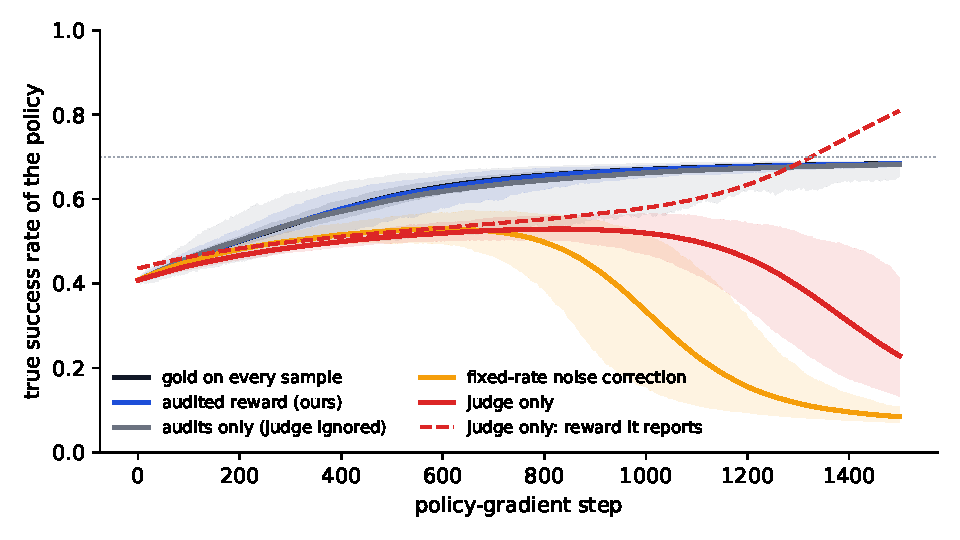
\includegraphics[width=0.82\linewidth]{fig1_sim_curves.pdf}
\caption{True success of the policy (mean and 95\% range over 200 seeds). The judge-only run reports a rising reward (dashed) while its true success collapses. Fixed-rate noise correction collapses faster. Audited rewards match gold on every sample with one eighth of the labels.}
\label{fig:curves}
\end{figure}

\begin{figure}[t]
\centering
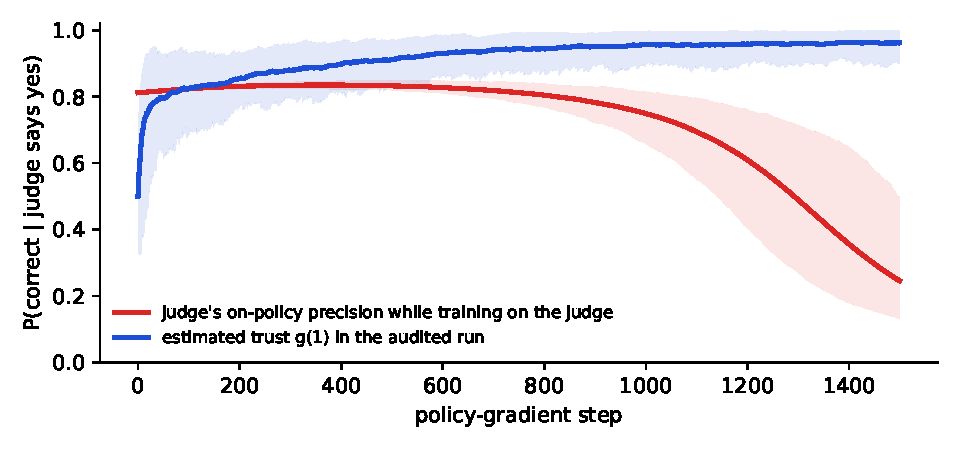
\includegraphics[width=0.82\linewidth]{fig2_sim_precision.pdf}
\caption{The judge's precision on the policy's own outputs falls from 0.81 to 0.25 when the judge pays the reward. This is the policy-dependent noise that fixed-rate corrections assume away. In the audited run, the estimated trust $g(\text{yes})$ tracks the precision of the audited policy.}
\label{fig:precision}
\end{figure}

\paragraph{The variance formula.}
At the initial policy with a fixed trust function, the empirical variance of $\rt$ over $4\times10^5$ draws is 1.192, and Equation~\eqref{eq:variance} predicts 1.199.

\paragraph{Label budget.}
We repeat the experiment with independent Bernoulli audits at rates from $1/8$ to $1/64$, 100 seeds each (Table~\ref{tab:sweep}, Figure~\ref{fig:sweep}). As labels become scarce, audits that ignore the judge lose both final success and stability, from 0.681 to 0.631, with the share of seeds above 0.6 falling from 99\% to 70\%. The audited reward stays close to the optimum, from 0.684 to 0.674, with 100\% to 95\% of seeds above 0.6. With 375 labels ($p=1/32$) the audited reward does as well as judge-free audits with 1{,}500 labels, which is what Theorem~\ref{thm:variance}(c) predicts for a judge that is informative on the policy's outputs.

\begin{table}[t]
\centering
\small
\caption{Label budget, Bernoulli audits, 100 seeds per cell. Final true success (standard deviation over seeds) and share of seeds ending above 0.6.}
\label{tab:sweep}
\begin{tabular}{@{}crcccc@{}}
\toprule
& & \multicolumn{2}{c}{Audits only, judge ignored} & \multicolumn{2}{c}{Audited reward} \\
\cmidrule(lr){3-4}\cmidrule(lr){5-6}
Audit rate & Gold labels & Final success & $>0.6$ & Final success & $>0.6$ \\
\midrule
$1/8$  & 1{,}500 & 0.681 (0.016) & 99\% & 0.684 (0.003) & 100\% \\
$1/16$ & 747     & 0.672 (0.038) & 93\% & 0.684 (0.004) & 100\% \\
$1/32$ & 375     & 0.656 (0.059) & 84\% & 0.682 (0.010) & 100\% \\
$1/64$ & 187     & 0.631 (0.082) & 70\% & 0.674 (0.034) & 95\% \\
\bottomrule
\end{tabular}
\end{table}

\begin{figure}[t]
\centering
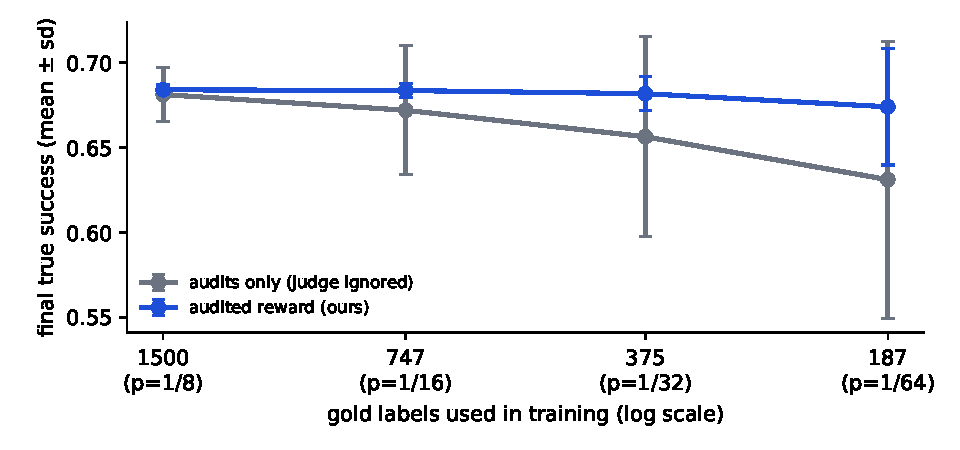
\includegraphics[width=0.78\linewidth]{fig3_sim_sweep.pdf}
\caption{Final true success (mean $\pm$ standard deviation over 100 seeds) against the number of gold labels used in training, on a log scale.}
\label{fig:sweep}
\end{figure}

\subsection{GRPO on GSM8K}
\label{sec:grpo}

\paragraph{Design.}
We train Qwen2.5-0.5B-Instruct \citep{qwen2024qwen25} on GSM8K \citep{cobbe2021gsm8k} with GRPO for 100 steps, 32 completions per step (four prompts with eight completions each). The judge is Qwen2.5-1.5B-Instruct, asked whether a completion's final answer is correct without seeing the answer key. The gold reward is exact match of the final number with the GSM8K answer. We compare four rewards. Gold on every sample uses 3{,}200 gold labels. The judge alone uses none. The audited reward and judge-free audits each audit one of the eight completions per prompt, chosen uniformly after generation, for 400 gold labels. The gold-only and judge-only runs are the ones reported by \citet{feryad2026rewardaudit}, with identical settings. Appendix~\ref{app:grpo} lists the hyperparameters.

\paragraph{Results.}
Table~\ref{tab:grpo} and Figure~\ref{fig:grpo} give the outcome. In this run the judge did not pull the policy away from the gold objective. All four rewards end at a true accuracy between 0.27 and 0.30, and with one seed and 320 completions per ten-step window these differences are within sampling noise (standard error about 0.025). The rewards differ in what they tell the trainer. Paid by the judge alone, the trainer sees a mean reward of 0.66 while the policy's true accuracy is 0.26, an overstatement of 0.40 that persists through training. In the audited run the judge accepts between 52\% and 66\% of completions while only 15\% to 30\% are correct (Figure~\ref{fig:grpo}c), and the trust $g(\text{yes})$ estimated from the audits stays between 0.26 and 0.40, close to the judge's low precision on this policy.

Both audited rewards are unbiased in practice. Over 400 reward calls, the mean of the reward minus the true accuracy is $-0.006$ for the audited reward and $-0.009$ for judge-free audits, and each uses 400 gold labels instead of 3{,}200. Because the judge explains little of the gold variation here, Theorem~\ref{thm:variance}(c) predicts only a modest gain from using it. The measured gain is of that size: the variance of the reward's error, per completion, is 0.686 for the audited reward and 0.857 for judge-free audits, a reduction of 20\%.

\begin{table}[t]
\centering
\small
\caption{GRPO on GSM8K, one seed, 100 steps. True accuracy is averaged over the first and last ten steps; the last two columns average over all 100 steps.}
\label{tab:grpo}
\begin{tabular}{@{}lrcccc@{}}
\toprule
& & \multicolumn{2}{c}{True accuracy} & \multicolumn{2}{c}{All steps} \\
\cmidrule(lr){3-4}\cmidrule(lr){5-6}
Reward used for training & Gold labels & First 10 & Last 10 & Reward seen & True accuracy \\
\midrule
Gold on every sample & 3{,}200 & 0.219 & 0.300 & 0.255 & 0.255 \\
Judge only & 0 & 0.222 & 0.303 & \textbf{0.657} & 0.255 \\
Audits only, judge ignored & 400 & 0.216 & 0.303 & 0.225 & 0.234 \\
Audited reward & 400 & 0.200 & 0.269 & 0.222 & 0.228 \\
\bottomrule
\end{tabular}
\end{table}

\begin{figure}[t]
\centering
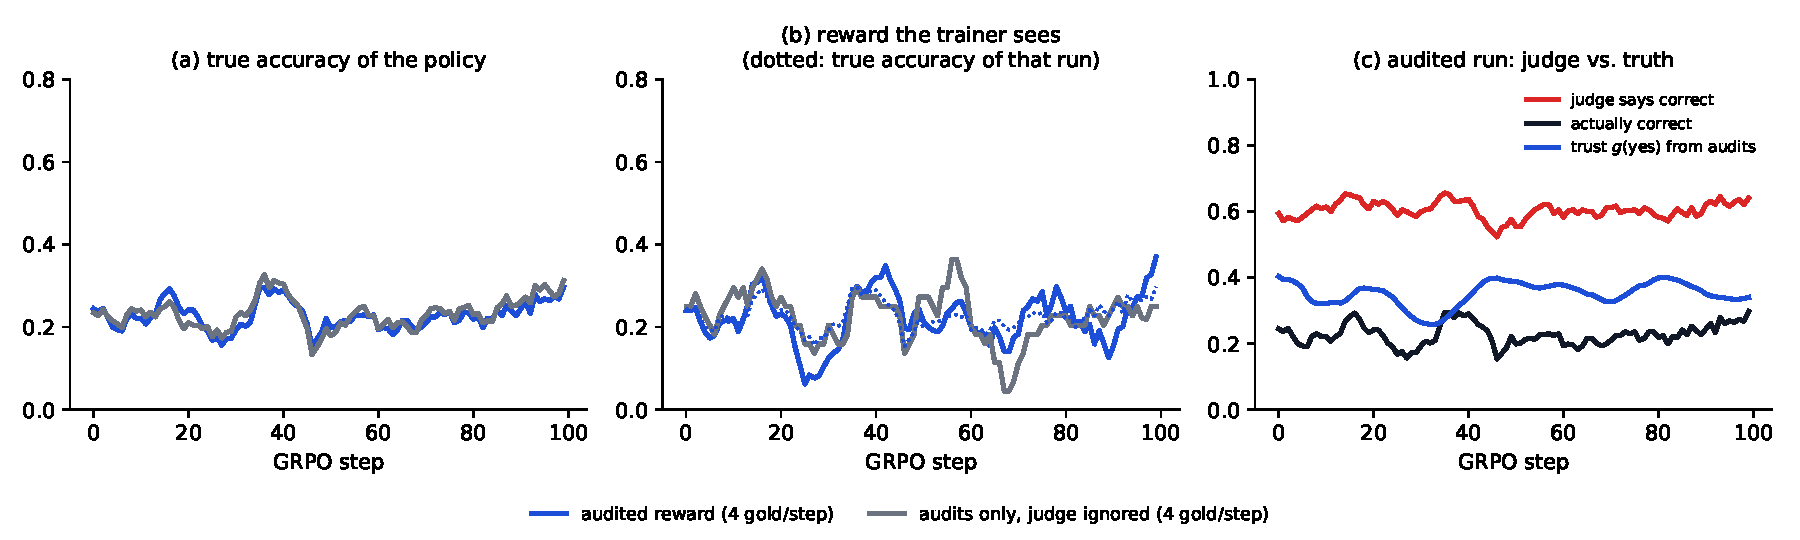
\includegraphics[width=\linewidth]{fig4_grpo.pdf}
\caption{GRPO on GSM8K, 11-step moving averages. (a) True accuracy of the policy under the four rewards. (b) The reward the trainer sees; dotted lines show the true accuracy of the judge-only and audited runs. The judge-only reward sits about 0.4 above the truth, while both audited rewards track it. (c) In the audited run, the share of completions the judge accepts, the share that are correct, and the trust $g(\text{yes})$ that the audits assign to an acceptance.}
\label{fig:grpo}
\end{figure}


\section{Discussion}
\label{sec:discussion}

The central point is that a grader's errors are not a fixed property of the grader. They are a property of the grader together with the distribution it is applied to, and in RL that distribution is chosen by an optimizer with an incentive to find the errors. Proposition~\ref{prop:impossible} turns this into a lower bound: no amount of judge data and no calibration set collected in advance can separate a real improvement from a hack the calibration set never saw. Theorem~\ref{thm:unbiased} shows that the fix does not require a better judge, only a small amount of gold placed by randomization after the policy has committed to its outputs.

The variance identity makes the trade-off concrete for a practitioner. The audit rate sets a variance multiplier of order $1/p$, and the judge reduces it by the share of gold variation it explains on the current policy. A judge that is good but exploitable is therefore still useful under audits: while it is accurate, it lets audits be rare, and once it is exploited its trust falls and the audits take over, without any change to the training code. The same audits estimate the judge's on-policy precision, which is a direct and interpretable measure of how much the judge is being gamed, and Proposition~\ref{prop:alarm} turns that estimate into an alarm with a guaranteed false-alarm rate.

Three practical rules follow. Audit decisions must be made after generation and must not depend on anything the policy can observe. Trust must be refitted on recent audits rather than fixed at the start. Audit rates may be raised wherever the judge and gold disagree most, which is Neyman's rule, and they may change at any time as long as they are set before the gold label is seen.

\section{Limitations}
\label{sec:limitations}

Unbiasedness is relative to the gold labeller. If the gold labels are themselves wrong, the method is unbiased for the labeller and not for the truth. The variance cost grows as $1/p$, so very low audit rates need a judge that is informative on the policy's own outputs. GRPO's standard-deviation scaling breaks exact unbiasedness, although the bias is a rescaling of each group's update. The simulation is a stylized four-armed bandit chosen to make the exploit explicit. The GRPO experiment uses a small policy, one task, one seed and 100 steps; in it the judge-only run did not lose true accuracy relative to gold, so the experiment tests label efficiency and the honesty of the reward signal rather than the rescue of a collapsing run. We have not tested multi-step agentic tasks, where an audit may need to cover a whole trajectory.

\section{Conclusion}
\label{sec:conclusion}

Reward hacking is label noise that the policy chooses. Corrections that fix the noise model before training cannot see it, and our impossibility result makes this precise. Randomly auditing a fraction of the policy's own outputs after they are written, and paying the judge's calibrated score plus an inverse-probability correction, removes the bias for every policy at an exact and computable variance cost. In a controlled exploit, this recovers the performance of full gold supervision with one eighth of the labels and stays stable at one thirty-second, where judge-free audits begin to fail. In GRPO on GSM8K, it keeps the training reward within 0.01 of the true accuracy where the judge alone overstates it by 0.40.

\subsubsection*{Reproducibility statement}
All code, logs and figures are in the \texttt{audited\_rewards/} folder of the public repository, and all paths below are relative to it. The simulation (\texttt{sim/bandit\_sim.py}, \texttt{sim/sweep.py}) runs on a laptop CPU in minutes and regenerates Tables~\ref{tab:sim} and \ref{tab:sweep} and Figures~\ref{fig:curves}--\ref{fig:sweep} from fixed seeds. The GRPO runs use one RTX~4090 for 40 to 50 minutes each, and the two audited runs together cost about 1.3 US dollars of cloud time; the training script logs per-step true accuracy, reward, judge verdicts and trust values, and \texttt{llm/analyze.py} produces Table~\ref{tab:grpo} and Figure~\ref{fig:grpo} from the logs.

\subsubsection*{Declaration of generative AI use}
The scientific contribution of this work is the author's own: the research idea, the questions studied, the study design and the interpretation of the results. Under the author's direction, a large language model (Claude, Anthropic) was used as a tool to implement and run the experiments, to draft and edit the manuscript text, and to script the verification of the reference list and the reported numbers. The author reviewed all content and takes full responsibility for the published article.

\subsubsection*{Broader impact statement}
The method is meant to make RL post-training more honest at low cost by preventing a model from being rewarded for fooling its grader. Its guarantee is only as good as the gold labels, and a developer could audit with a weak gold labeller and claim the guarantee anyway. We recommend reporting the gold source, the audit rate and the on-policy precision of the judge alongside any result trained with audited rewards.

\bibliography{refs}
\bibliographystyle{tmlr}

\appendix

\section{Simulation settings}
\label{app:sim}

\begin{table}[h]
\centering
\small
\begin{tabular}{@{}ll@{}}
\toprule
Setting & Value \\
\midrule
Gold success per strategy $\mu$ & $(0.50, 0.20, 0.05, 0.70)$ \\
Judge true-positive rate per strategy & $(0.90, 0.90, 0.95, 0.80)$ \\
Judge false-positive rate per strategy & $(0.10, 0.10, 0.95, 0.05)$ \\
Initial logits & $(1.0, 1.0, -1.5, 0.3)$; exploit mass about 3\% \\
Samples per step $G$ & 8 \\
Steps, learning rate & 1{,}500, 0.05 \\
Seeds & 200 (main), 100 per cell (label budget) \\
Audit design (main) & one of $G$ samples, uniform, after sampling; $p=1/8$ \\
Audit design (label budget) & independent Bernoulli, $p\in\{1/8,1/16,1/32,1/64\}$ \\
Trust $g(j)$ & running $P(y=1\mid j)$, forgetting factor 0.98, prior weight 2 \\
Fixed-rate correction & rates estimated from 1{,}500 gold labels on the initial policy \\
\bottomrule
\end{tabular}
\end{table}

\section{GRPO settings}
\label{app:grpo}

\begin{table}[h]
\centering
\small
\begin{tabular}{@{}ll@{}}
\toprule
Setting & Value \\
\midrule
Policy & Qwen2.5-0.5B-Instruct \\
Judge & Qwen2.5-1.5B-Instruct, no answer key, yes/no verdict \\
Data & GSM8K training split, shuffled with the run seed \\
Steps & 100 \\
Completions per step & 32 (4 prompts $\times$ 8 completions) \\
Learning rate, KL coefficient $\beta$ & $5\times10^{-6}$, 0.04 \\
Maximum completion length & 200 tokens \\
Audits & one of 8 completions per prompt, uniform, after generation \\
Trust $g(j)$ & running $P(y=1\mid j)$, forgetting factor 0.98, prior weight 2 \\
Hardware & one NVIDIA RTX 4090 \\
\bottomrule
\end{tabular}
\end{table}

\end{document}

